\newpage
\section{The Pinwheel Tiling}

In this activity, we are going to investigate a very special rep-tile,
the \textit{pinwheel tiling}.\index{pinwheel tiling}

\begin{prob}
The pinwheel tiling is based on the following triangle:
\[
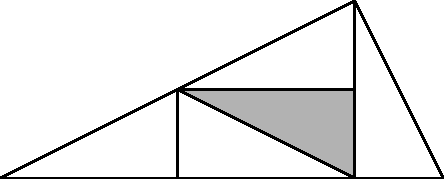
\includegraphics{../graphics/pinwheelBase.pdf}
\]
If the shortest side of the shaded triangle has a length of 1 unit and this is a rep-5-tile,
what are the lengths of the other sides? What type of triangle is
this?
\end{prob}

\begin{prob}
Each time we ``inflate'' the pinwheel rep-tile, we view the new, larger
triangle as being the shaded triangle in our base rep-tile. Inflate
the triangle below two times.
\[
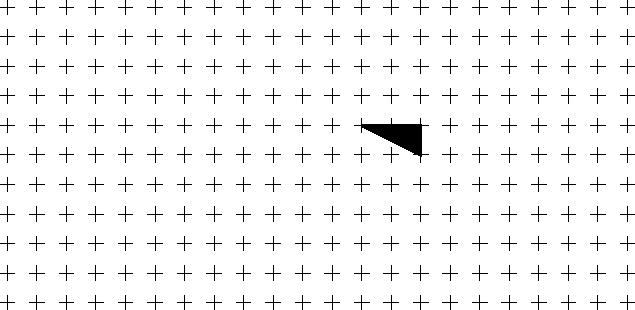
\includegraphics{../graphics/pinwheelInflate.pdf}
\]
Check with your friend to see that you get the same result.
\end{prob}


\begin{prob}
For the rep-tile above, compute the perimeter and area. How does this
relate to the perimeter and area of the larger triangle?
\end{prob}

\break

\begin{prob}
In the picture below, shade in (using colored pencils) the various
inflations of the shaded pinwheel rep-tile.
\[
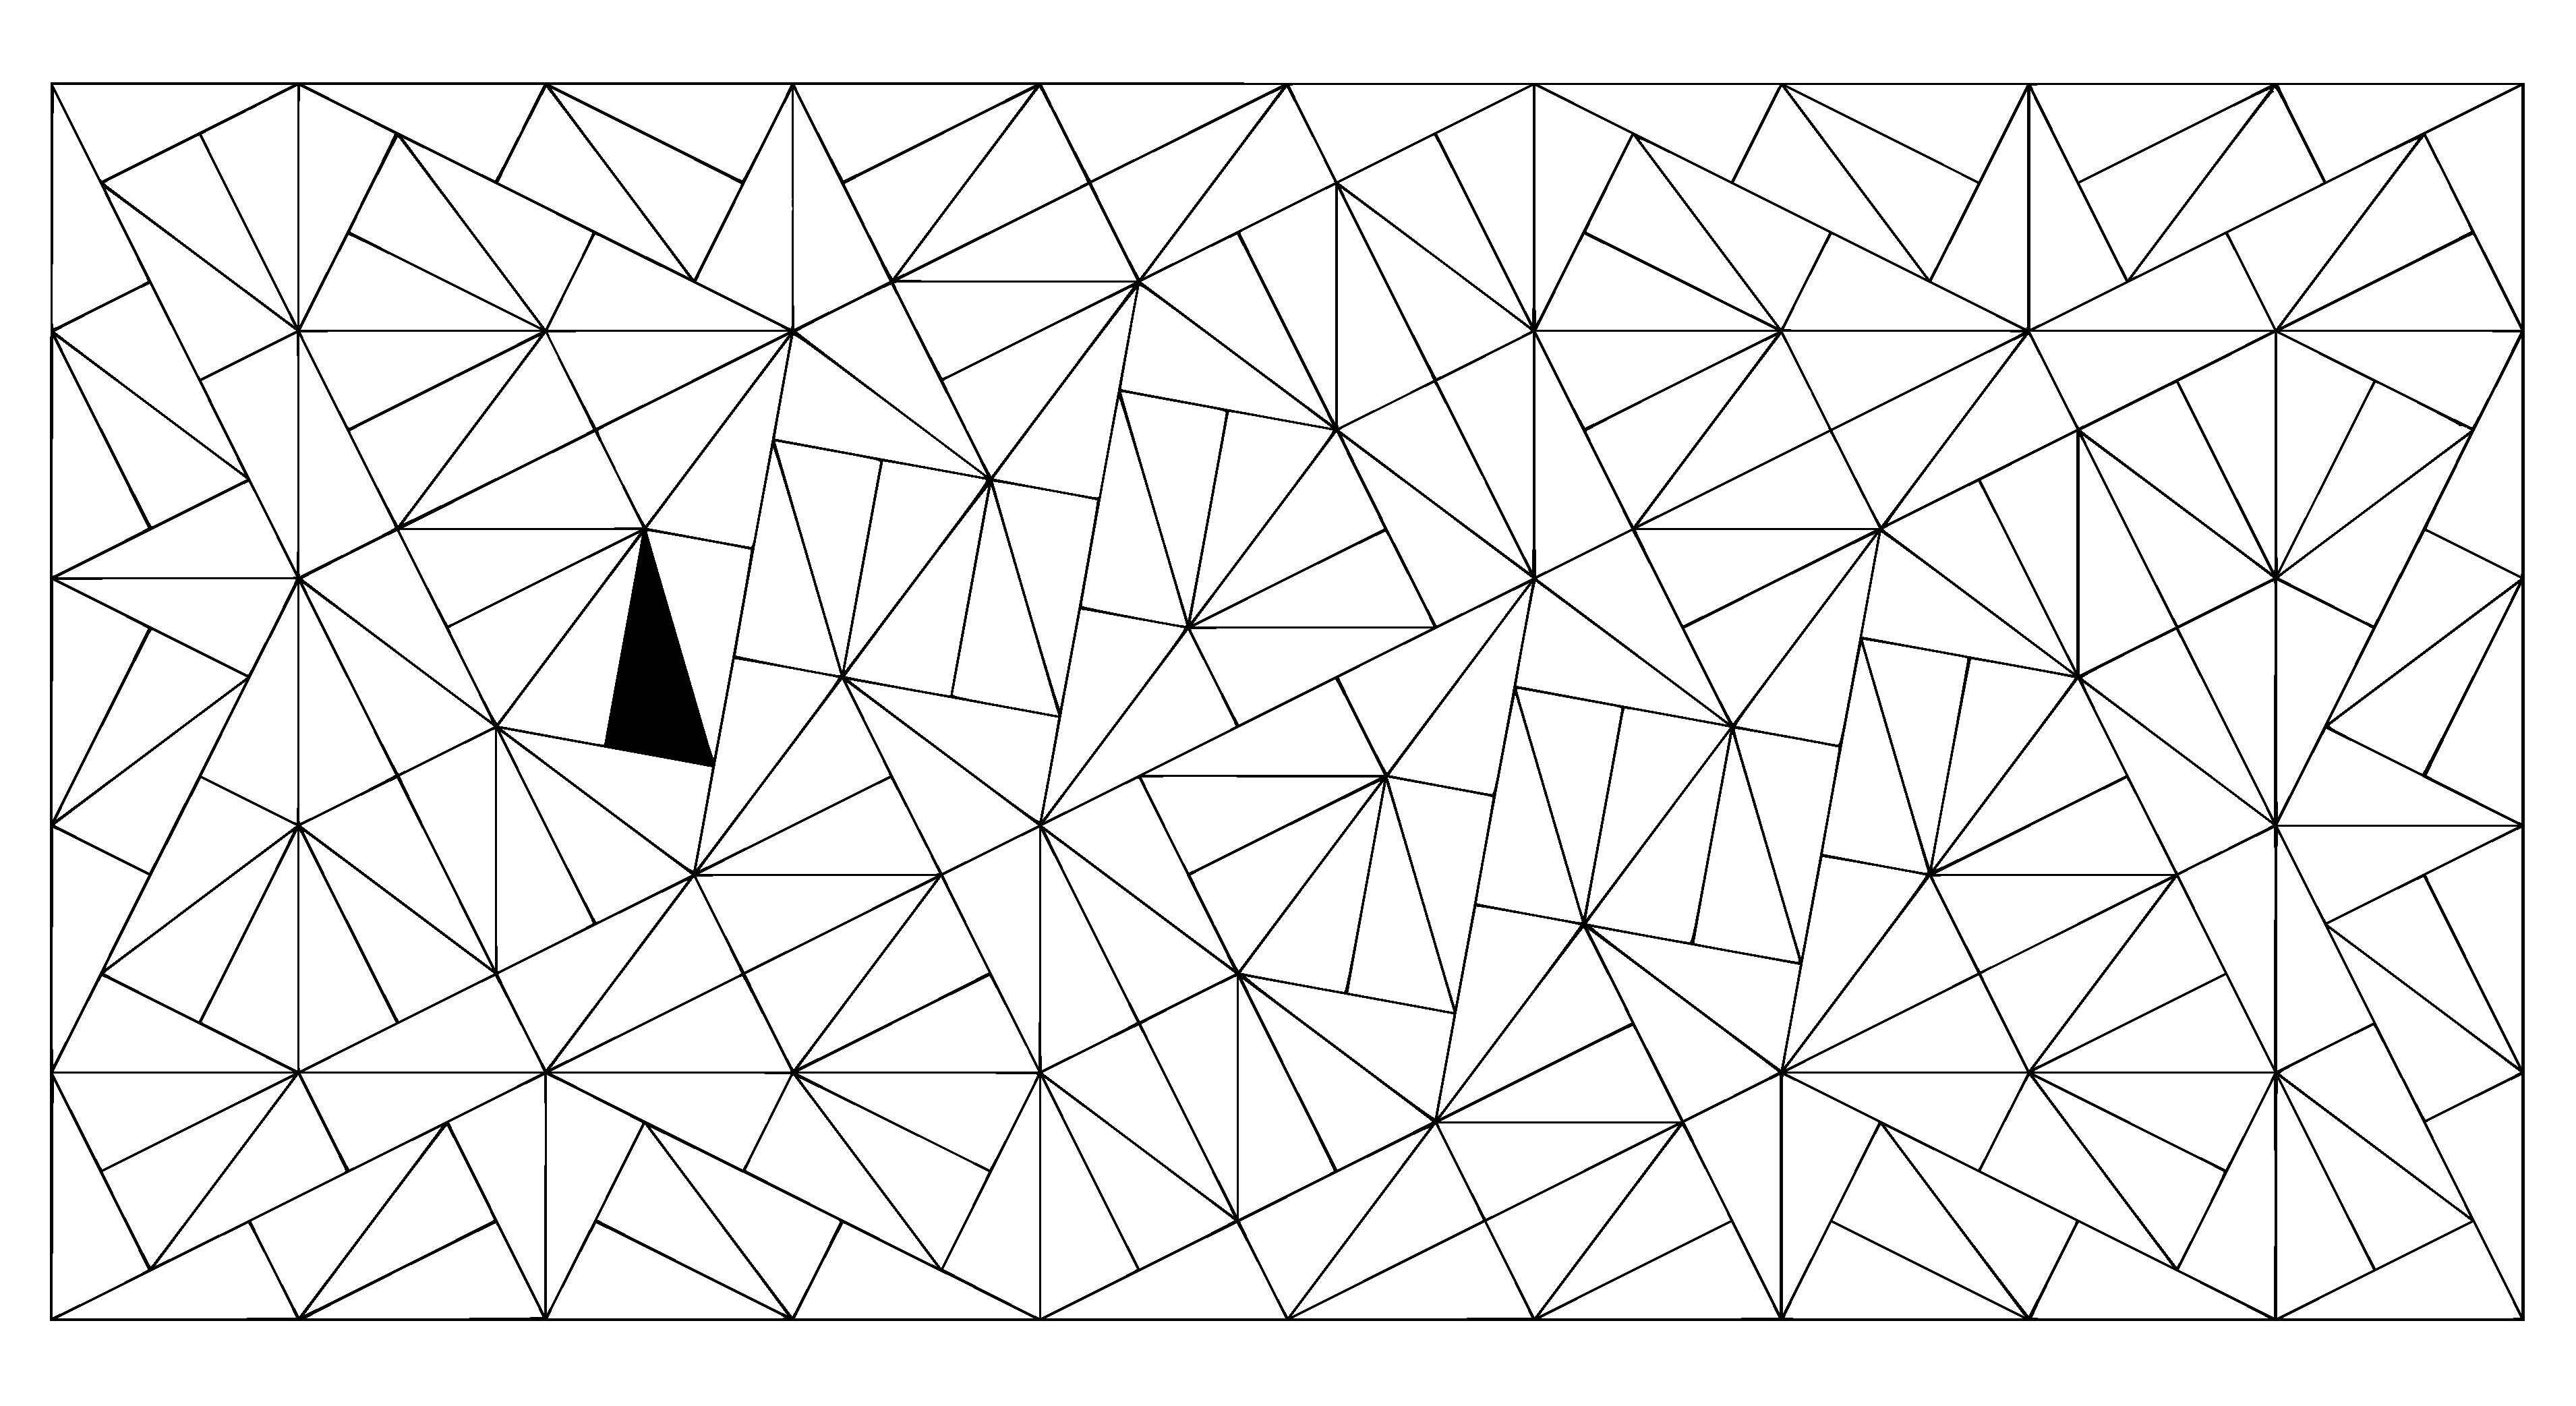
\includegraphics[width=\textwidth]{../graphics/pinwheel1.pdf}
\]
\end{prob}


\begin{prob}
While only the shaded triangle above is used to ``inflate'' the
pinwheel rep-tile, every triangle is part of \textbf{some}
inflation. In the picture below, shade in (using colored pencils) the
various inflations containing the shaded pinwheel rep-tile.
\[
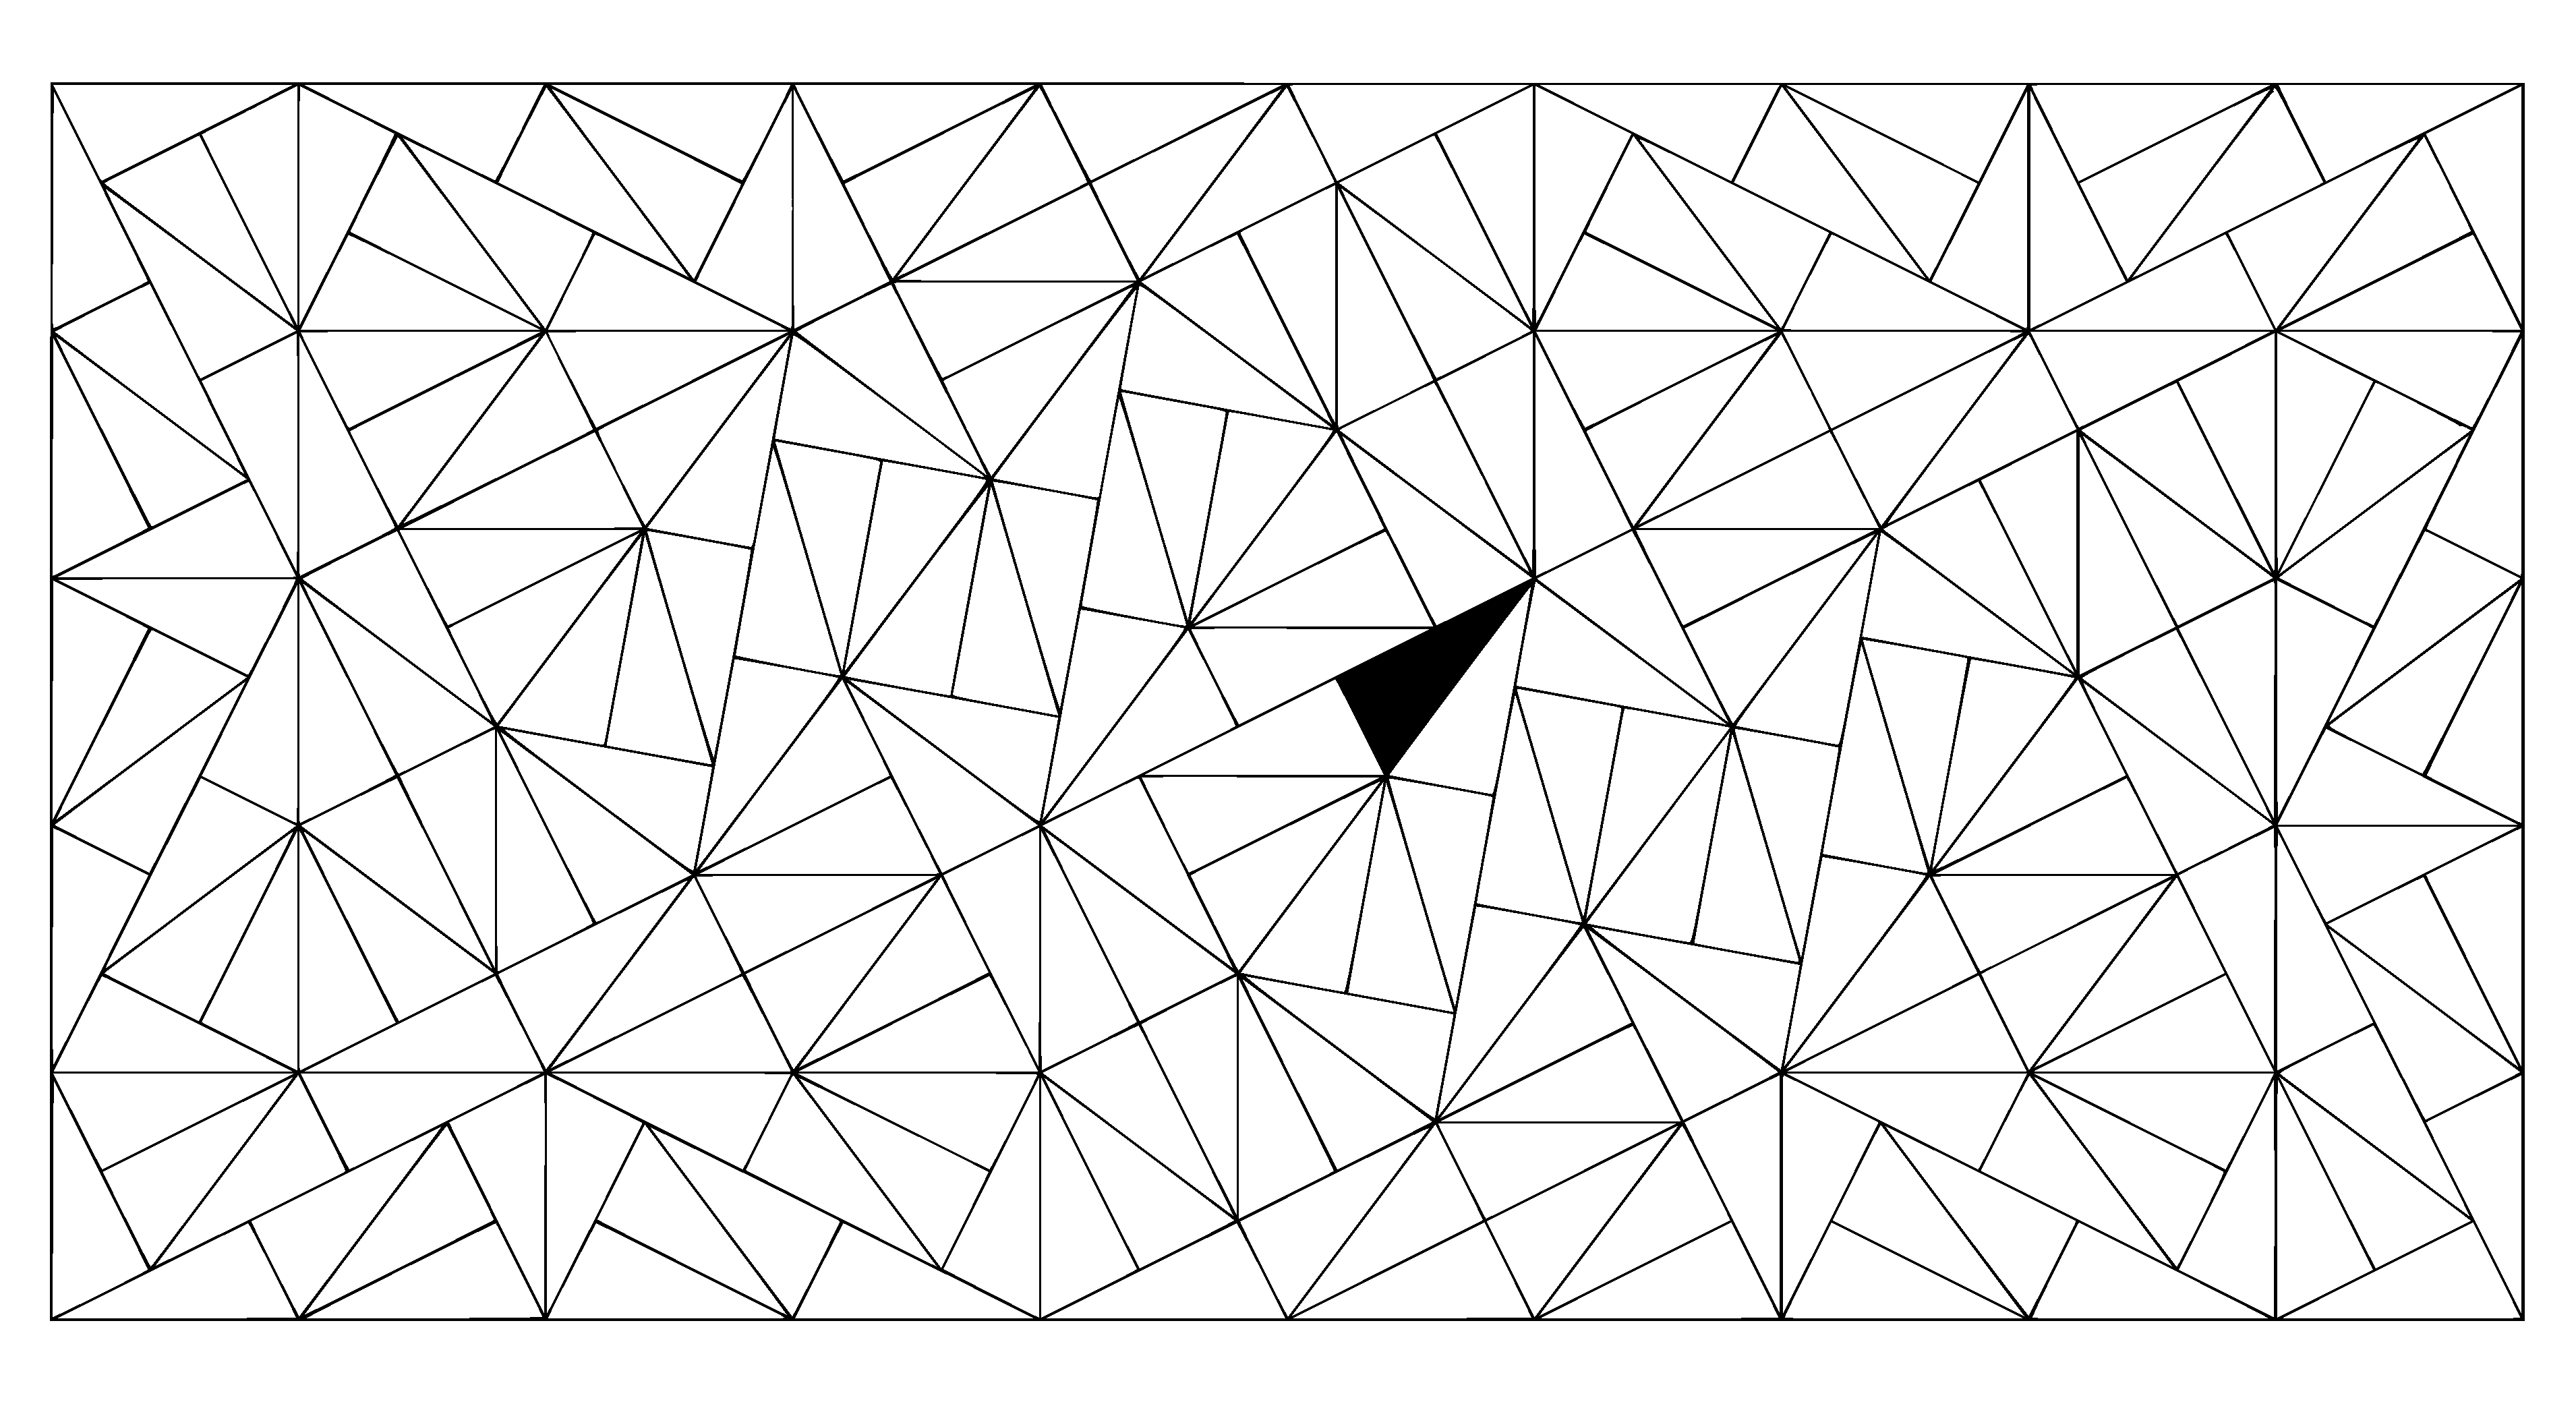
\includegraphics[width=\textwidth]{../graphics/pinwheel2.pdf}
\]
\end{prob}


\break

\begin{prob}
In the picture below, shade in (using colored pencils) the
various inflations containing the shaded pinwheel rep-tile.
\[
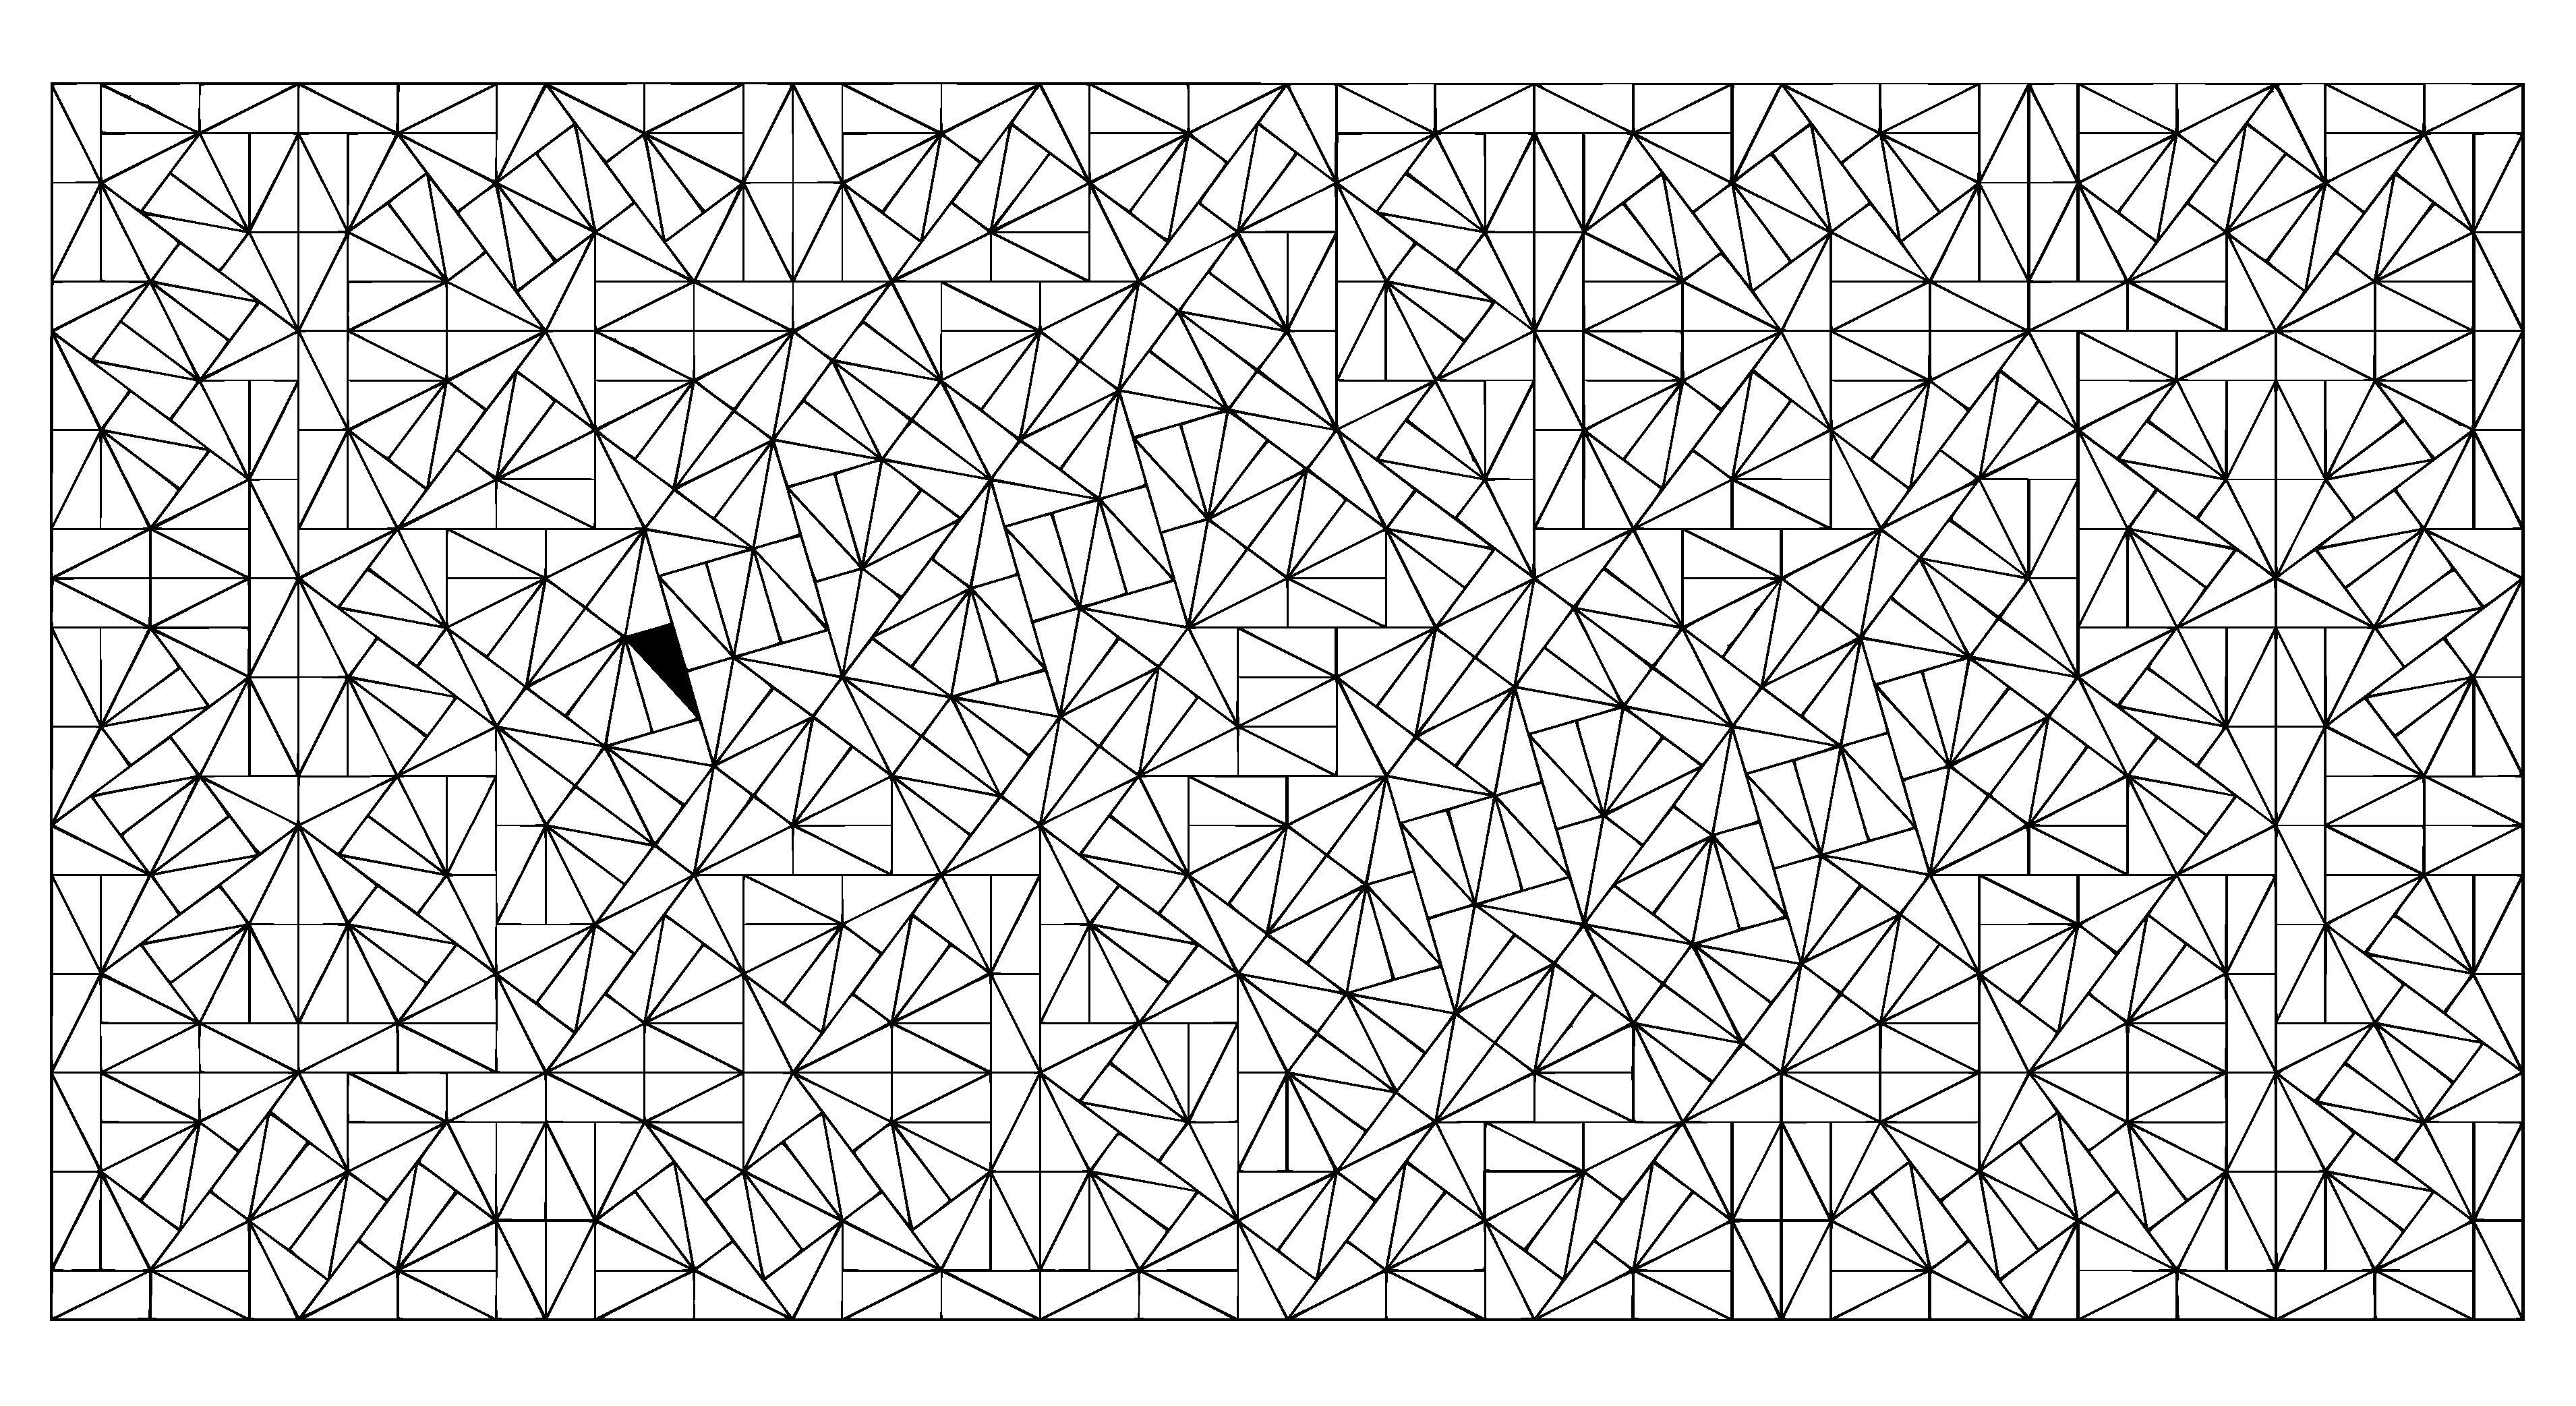
\includegraphics[width=\textwidth]{../graphics/pinwheel3.pdf}
\]
\end{prob}

\begin{prob}
While only the shaded triangle above is used to ``inflate'' the
pinwheel rep-tile, every triangle is part of \textbf{some}
inflation. In the picture below, shade in (using colored pencils) the
various inflations containing the shaded pinwheel rep-tile.
\[
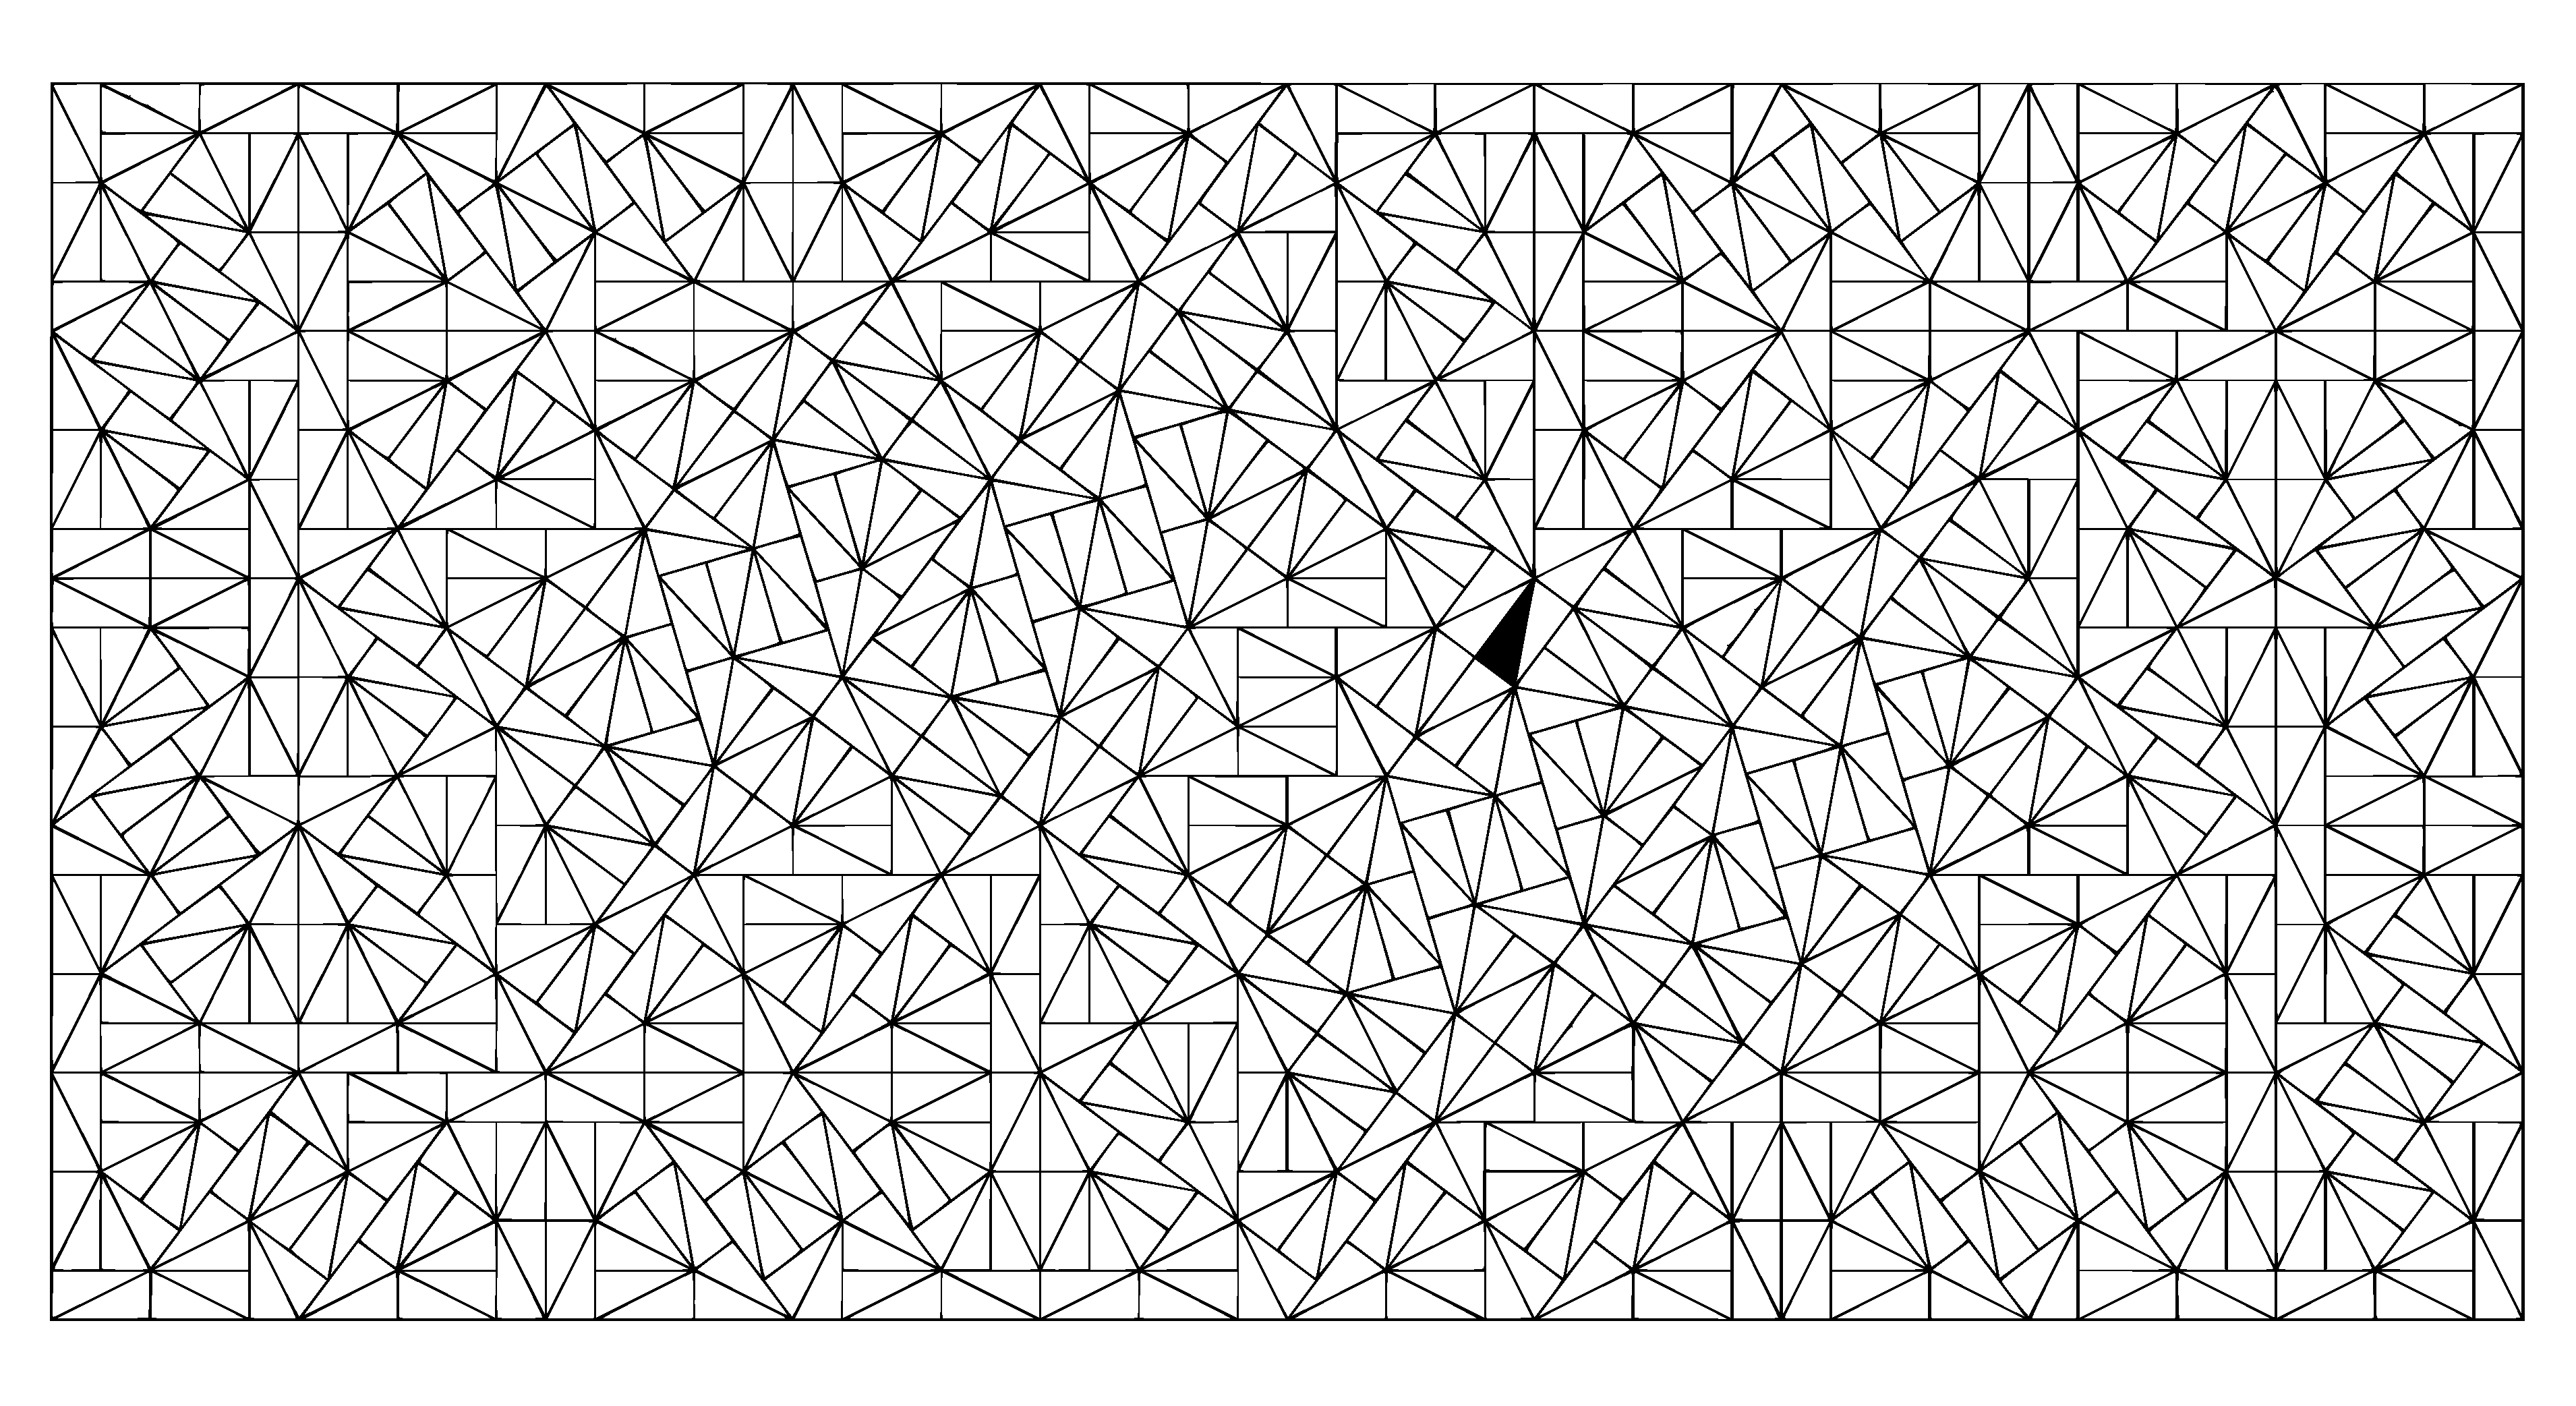
\includegraphics[width=\textwidth]{../graphics/pinwheel4.pdf}
\]
\end{prob}


\break

We claim that the pinwheel tiling has no symmetry through any
isometry---yet it still has symmetry of scale.


\begin{prob}
Explain why any triangle in a pinwheel tiling is necessarily a part of
one, and only one, inflation.
\end{prob}


\begin{prob}
Suppose there was an isometry that moved one triangle to another. What
would that say about an inflation that contained them both? Why would
that contradict the problem above?
\end{prob}


\begin{prob}
The pinwheel tiling has been used in the design of several famous
buildings---which ones?
\end{prob}
